\chapter{Konvergenz von Funktionen}

\setcounter{section}{5}
\setcounter{subsection}{0}
\setcounter{subsubsection}{1}
\setcounter{secnumdepth}{3}
\subsection{Funktionen und Folgen}
\href{https://youtu.be/uTHOemsexgc}{Video 01}\\
Sei $ f:\mathbb{R}\supset \mathbb{D}_f\longmapsto \mathbb{R} $ eine Funktion und $ (x_n)_{n\in\mathbb{N}} $ eine reelle Folge, dann ist:\\
\begin{align*}
\bigg(f(x_n)\bigg)_{n\in\mathbb{N}}=f(x_0), f(x_1)\ldots
\end{align*}
auch eine reelle Zahlenfolge.\vspace*{4mm}\\
Beispiel:\\
Sei:\\
$ f:\mathbb{R}\longmapsto [0,\infty[ $ mit $ f(x)=x^2 $ und $x_n= \big(\frac{1}{n}\big)_{n\in\mathbb{N}\backslash\{0\}} $\\
Dann ist:\\
$ f\big((x_n)\big)_{n\in\mathbb{N}\backslash\{0\}} =\big((\frac{1}{n})^2\big)_{n\in\mathbb{N}\backslash\{0\}}=1,\frac{1}{4},\frac{1}{9},\frac{1}{16}\ldots$\\
\begin{center}

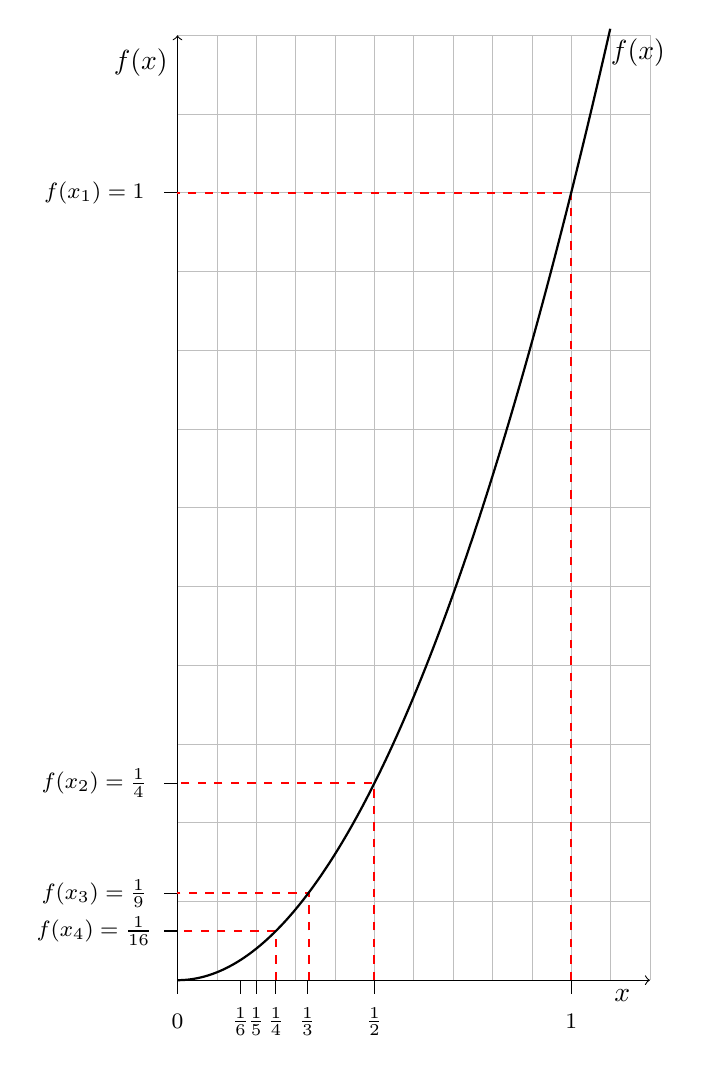
\begin{tikzpicture}[yscale=10,xscale=5]

% Gitternetzlinien
\draw[xstep=0.1cm, ystep=0.1cm, very thin, color=lightgray] (0,1.2) grid (1.2,0);
% x-Achse
\draw[->] (0,0) -- (1.2,0) node[below,xshift=-1em] {$x$}; 
%Zahlen auf x-Achse

% y-Achse 
\draw[->] (0,0) -- (0,1.2) node[left,yshift=-1em] {$f(x)$};%node[above left]
%Zahlen auf y-Achse

%\foreach \y in {1,...,1}
%\draw[shift={(0,\y)},color=black] (2pt,0pt) -- (-2pt,0pt) node[left] {\footnotesize $\y$};
%Ursprung
\draw[color=black] (1,0) node[yshift=-1.5em] {\footnotesize $1$};
\draw[color=black] (1,0) --(1,-0.5pt);
\draw[color=black] (0,0) node[yshift=-1.5em] {\footnotesize $0$};
\draw[color=black] (0,0) --(0,-0.5pt);
\draw[color=black] (0.5,0) node[yshift=-1.5em] {\footnotesize $\frac{1}{2}$};
\draw[color=black] (0.5,0) --(0.5,-0.5pt);

\draw[color=black] (0.25,0) node[yshift=-1.5em] {\footnotesize $\frac{1}{4}$};
\draw[color=black] (0.25,0) --(0.25,-0.5pt);

\draw[color=black] (0.33,0) node[yshift=-1.5em] {\footnotesize $\frac{1}{3}$};
\draw[color=black] (0.33,0) --(0.33,-0.5pt);
\draw[color=black] (0.2,0) node[yshift=-1.5em] {\footnotesize $\frac{1}{5}$};
\draw[color=black] (0.2,0) --(0.2,-0.5pt);
\draw[color=black] (0.16,0) node[yshift=-1.5em] {\footnotesize $\frac{1}{6}$};
\draw[color=black] (0.16,0) --(0.16,-0.5pt);
\draw[color=black] (0,0.25) node[xshift=-3em] {\footnotesize $f(x_2)=\frac{1}{4}$};
\draw[color=black] (0,0.25) --(-1pt,0.25);
\draw[color=black] (0,0.11) node[xshift=-3em] {\footnotesize $f(x_3)=\frac{1}{9}$};
\draw[color=black] (0,0.11) --(-1pt,0.11);
\draw[color=black] (0,0.0625) node[xshift=-3em] {\footnotesize $f(x_4)=\frac{1}{16}$};
\draw[color=black] (0,0.0625) --(-1pt,0.0625);
\draw[color=black] (0,1) node[xshift=-3em] {\footnotesize $f(x_1)=1$};
\draw[color=black] (0,1) --(-1pt,1);

\draw[color=red,thick,dashed] (1,0) --(1,1)--(0,1);
\draw[color=red,thick,dashed] (0.5,0) --(0.5,0.25)--(0,0.25);
\draw[color=red,thick,dashed] (0.25,0) --(0.25,1/16)--(0,1/16);
\draw[color=red,thick,dashed] (1/3,0) --(1/3,1/9)--(0,1/9);
\draw[thick,color=black] plot[samples=200, domain=0:1.1] 
(\x,{\x*\x}) node[below, xshift=1em]{$f(x)$};



\end{tikzpicture}\
\end{center}
Die Zahlenfolge $ f\big((x_n)\big)_{n\in\mathbb{N}\backslash\{0\}} $ konvergiert auf der y-Achse bis zum Grenzwert 0 und die Folge $ (\frac{1}{n})_{n\in\mathbb{N}\backslash\{0\}} $ konvergiert ebenfalls auf der x-Achse gegen den Grenzwert 0.\\
\subsection{Konvergenz von Funktionen}
\href{https://youtu.be/JM5KwRHuPKc}{Video 02}\\
Definition:\\
Sei $ f:\mathbb{R}\supset \mathbb{D}_f\longmapsto \mathbb{R} $ eine Funktion, dann gilt:\\
Die Funktion $ f $ hat für $ x $ gegen $ x_0 $ den Grenzwert $ y_0 $, wenn für jede Folge in $ (x_n)_{n\in\mathbb{N}} $ in $ \mathbb{D}_f\backslash \{x_0\} $, mit $ \lim\limits_ {n\to\infty}x_n=x_0 $, der Grenzwert $ \lim\limits_ {n\to\infty} f(x_n) $ exestiert und gleich $ y_0 $ ist.\vspace*{2mm}\\
Beispiel:\\
Sei $ f: \mathbb{R}\longmapsto \mathbb{R} $ mit $ f(x)=2x $ und $ x_0=2\Rightarrow y_0=4 $ und die Folge $ x_n=(\frac{1}{n})+2 $.\\
Es gilt:
\begin{align*}
\lim\limits_ {n\to\infty} \frac{1}{n}+2=2=x_0
\end{align*}
Ebenso gilt:\\
\begin{align*}
\lim\limits_ {n\to\infty} f(x_n)=2\bigg(\frac{1}{n}+2\bigg)=4=y_0
\end{align*}
Diese Aussage gilt jetzt genau für diese eine Folge, aber nicht für alle!\\
Jede Folge mit dem Grenzwert 2 muss ergeben, dass der Grenzwert existiert und $ \lim\limits_ {n\to\infty} f(x_n)=y_0 $ ist:\\
\begin{center}

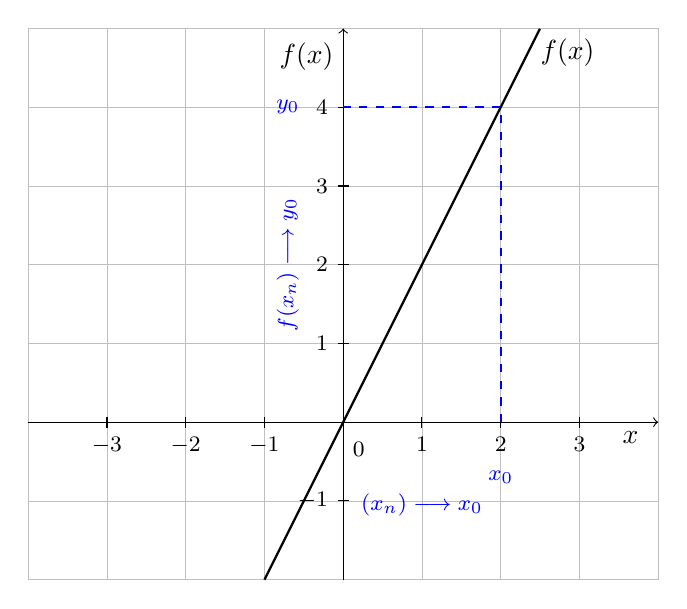
\begin{tikzpicture}

% Gitternetzlinien
\draw[xstep=1cm, ystep=1cm, very thin, color=lightgray] (-4,5) grid (4,-2);
% x-Achse
\draw[->] (-4,0) -- (4,0) node[below,xshift=-1em] {$x$}; 
%Zahlen auf x-Achse
\foreach \x in {-3,...,-1}
\draw[shift={(\x,0)},color=black] (0pt,2pt) -- (0pt,-2pt) node[below] {\footnotesize $\x$};
\foreach \x in {1,...,3}
\draw[shift={(\x,0)},color=black] (0pt,2pt) -- (0pt,-2pt) node[below] {\footnotesize $\x$};
% y-Achse 
\draw[->] (0,-2) -- (0,5) node[left,yshift=-1em] {$f(x)$};%node[above left]
%Zahlen auf y-Achse
\foreach \y in {-1,...,-1}
\draw[shift={(0,\y)},color=black] (2pt,0pt) -- (-2pt,0pt) node[left] {\footnotesize $\y$};
\foreach \y in {1,...,4}
\draw[shift={(0,\y)},color=black] (2pt,0pt) -- (-2pt,0pt) node[left] {\footnotesize $\y$};
%Ursprung
\draw[color=black] (0pt,-10pt) node[right] {\footnotesize $0$};



\draw[thick,color=black] plot[samples=200, domain=-1:2.5] 
(\x,{2*\x}) node[below, xshift=1em]{$f(x)$};

\draw[color=blue] (2,0) node[yshift=-20] {\footnotesize $x_0$};
\draw[color=blue] (1,0) node[yshift=-30] {\footnotesize $(x_n)\longrightarrow x_0$};
\draw[color=blue] (0,4) node[xshift=-20] {\footnotesize $y_0$};
\draw[color=blue] (0,2) node[xshift=-20,rotate=90] {\footnotesize $f(x_n)\longrightarrow y_0$};
\draw[color=blue,dashed,thick] (2,0)--(2,4)--(0,4);
\end{tikzpicture}\\
\end{center}
Bemerkung:\\
$ x_0 $ muß nicht notwendigerweise in $ \mathbb{D}_f $ sein.\\
Wir betrachten auch $ \lim\limits_ {x\to\pm\infty}f(x) $. Z.B.($ \lim\limits_ {x\to\infty}f(x)=\frac{1}{\frac{1}{x}+1} $)\\
\subsubsection{Beispiel zum Nachweis der Konvergenz von Funktionen-Teil I}
\href{https://youtu.be/sLrX5Et79Kg}{Video 03}\\
(i)\;\;$f:\mathbb{R}\longmapsto[0,\infty[$ für $ f(x)=x^2 $\\
\begin{quote}
	Zeige:\\
	\begin{align*}
	\lim\limits_ {x\to 0}f(x)=\lim\limits_ {x\to 0}x^2=0\\
	\end{align*}
	\textbf{Fehler: Falsche Betrachtung!}\\
	Betrachte:\\ Nullfolge $ (\frac{1}{n})_{n\in\mathbb{N}} $\\
	Es gilt:
	\begin{align*}
	\lim\limits_ {n\to \infty}f(x_n)=\lim\limits_ {n\to \infty}\frac{1}{n}=0
	\end{align*}
	Dies reicht nicht, weil $ (\frac{1}{n})_{n\in\mathbb{N}} $ eine konkrete Folge ist und nicht alle Nullfolgen repräsentieren!!\vspace*{4mm}\\
	\textbf{Richtig:}
	Man nehme eine beliebige Folge:\\
	Sei $ (x_n) $ eine beliebige Folge für die gilt $ \lim\limits_ {n\to\infty}(x_n)=0 $\\
	Betrachte:\\
	\begin{align*}
	\lim\limits_ {n\to\infty}f(x_n)=\lim\limits_ {n\to\infty}x_{n}^2=\lim\limits_ {n\to\infty}x_n\lim\limits_ {n\to\infty}x_n=0\cdot0=0
	\end{align*}
	D.h.:\\
	Der $ \lim\limits_ {n\to\infty}f(x_n) =0$ für jede beliebige Nullfolge.\\
	\begin{align*}
	\Rightarrow\lim\limits_ {x\to 0}f(x)=\lim\limits_ {x\to 0}x^2=0
	\end{align*}
\end{quote}
(ii)\;\;$ \lim\limits_ {x\to 2}x^2=4 $\\
\begin{quote}
Wähle eine beliebige Folge $(x_n)_{n\in\mathbb{N}}$ für die gilt $ \lim\limits_ {n\to\infty}x_n=2 $ .
\begin{align*}
\lim\limits_ {n\to\infty}(x_n)^2=\lim\limits_ {n\to\infty}x_n\lim\limits_ {n\to\infty}x_n=2\cdot2=4
\end{align*}
\end{quote}
(iii) \;\;$\lim\limits_ {x\to 4}\frac{1}{x}=\frac{1}{4}$\\
\begin{quote}
Wähle eine beliebige Folge $(x_n)_{n\in\mathbb{N}}$ für die gilt $ \lim\limits_ {n\to\infty}x_n=4 $ .\\
\begin{align*}
\lim\limits_ {n\to\infty}\frac{1}{x_n}=\frac{\lim\limits_ {n\to\infty}1}{\lim\limits_ {n\to\infty}x_n}=\frac{1}{4}
\end{align*}
\end{quote}
\subsubsection{Beispiel zum Nachweis der Konvergenz von Funktionen-Teil II}
\href{https://youtu.be/in86heC1gIQ}{Video 04}\\
(i)\;\; $ f_1(x):\mathbb{R}\longmapsto \mathbb{R} $ mit $ f(x)=2x $\\
\begin{quote}
	\begin{align*}
	\lim\limits_ {x\to\infty} f_1(x)=\lim\limits_ {x\to\infty}2x=0\\
	\end{align*}
\end{quote}
(ii)\;\;$ f_2:\mathbb{R}\backslash\{0\}\longmapsto\mathbb{R} $ mit $ f(x) =\frac{2x}{x}$\\
\begin{quote}
	\begin{align*}
	\lim\limits_ {x\to\infty}f_2(x)=\lim\limits_ {x\to\infty}\frac{2x}{x}=0
	\end{align*}
	Null kann hier nicht eingesetzt werden! Der Grenzwert ist keine Funktion!\\
\end{quote}
(iii)\;\;$ \lim\limits_ {x\to\infty}\sin(x) $\\
\begin{quote}
	\begin{center}
		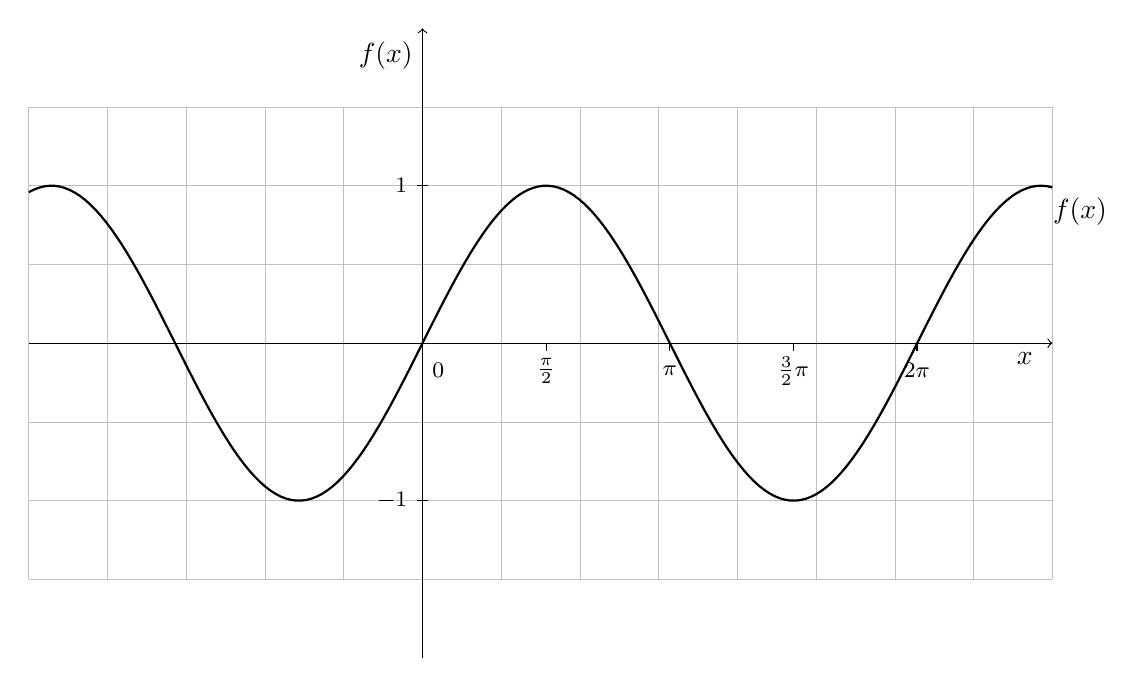
\begin{tikzpicture} [yscale=2]
		
		% Gitternetzlinien
		\draw[xstep=1cm, ystep=0.5cm, very thin, color=lightgray] (-5,1.5) grid (8,-1.5);
		% x-Achse
		\draw[->] (-5,0) -- (8,0) node[below,xshift=-1em] {$x$}; 
		%Zahlen auf x-Achse
		%\foreach \x in {-1,...,-6}
		%\draw[shift={(\x,0)},color=black] (0pt,2pt) -- (0pt,-2pt) node[below] {\footnotesize $\x$};
		%\foreach \x in {1,...,5}
		%\draw[shift={(\x,0)},color=black] (0pt,2pt) -- (0pt,-2pt) node[below] {\footnotesize $\x$};
		% y-Achse 
		\draw[->] (0,-2) -- (0,2) node[left,yshift=-1em] {$f(x)$};%node[above left]
		%Zahlen auf y-Achse
		\foreach \y in {-1,...,-1}
		\draw[shift={(0,\y)},color=black] (2pt,0pt) -- (-2pt,0pt) node[left] {\footnotesize $\y$};
		\foreach \y in {1,...,1}
		\draw[shift={(0,\y)},color=black] (2pt,0pt) -- (-2pt,0pt) node[left] {\footnotesize $\y$};
		%Ursprung
		\draw[color=black] (0pt,-5pt) node[right] {\footnotesize $0$};
		
		\draw[color=black] (3.14/2,-5pt) node {\footnotesize $\frac{\pi}{2}$};
		\draw[color=black] (3.14/2,0) --(3.14/2,-0.05);
		
		\draw[color=black] (3.14,-5pt) node {\footnotesize $\pi$};
		\draw[color=black] (3.14,0) --(3.14,-0.05);
		
		\draw[color=black] (3.14*2,-5pt) node {\footnotesize $2\pi$};
		\draw[color=black] (3.14*2,0) --(3.14*2,-0.05);
		
		\draw[color=black] (3.14*3/2,-5pt) node {\footnotesize $\frac{3}{2}\pi$};
		\draw[color=black] (3.14*3/2,0) --(3.14*3/2,-0.05);
		\draw[thick,color=black] plot[samples=200, domain=-5:8] 
		(\x,{sin(\x r)}) node[below, xshift=1em]{$f(x)$};
		
		
		
		\end{tikzpicture}\\
	\end{center}
Die Frage: Wohin läuft die Funktion?\\
Betrachte:\\
\textbullet \;\;Die Folge $ (n\cdot\pi)_{n\in\mathbb{N}} $\\
\begin{quote}
	Offensichtlich gilt:\\
	\begin{align}
	&\lim\limits_ {n\to\infty} n\cdot\pi=\infty \nonumber\\
	&\lim\limits_ {n\to\infty}(\sin(n\cdot\pi))=0
	\end{align}
\end{quote}
\textbullet \;\;Die Folge $ (\frac{\pi}{2}+n\cdot\pi)_{n\in\mathbb{N}} $\\
\begin{quote}
	Offensichtlich gilt:\\
	\begin{align}
	&\lim\limits_ {n\to\infty}\bigg(\frac{\pi}{2}+n\cdot\pi\bigg)=\infty\nonumber \\
	&\lim\limits_ {n\to\infty}\sin\bigg(\frac{\pi}{2}+n\cdot\pi\bigg)=(-1)^n=+1,-1,+1\ldots
	\end{align}
\end{quote}
Der Grenzwert von $ \lim\limits_ {n\to\infty}(-1)^n $ existiert nicht, also kann auch der Grenzwert $ \lim\limits_ {n\to\infty}\sin(x) $ nicht existieren.
Nach der Definition (Konvergenz von Folgen) existiert kein Grenzwert. Der Grenzwert von (V.1) muß gleich den Grenzwert von (V.2) sein.\vspace*{2mm}\\
\end{quote}
(iv)\;\;$ \lim\limits_ {x\to\infty} x=\infty$\\
\begin{quote}
	Die Folge divergiert in das positive Unendliche.\\
\end{quote}
(v)\;\;$\lim\limits_ {n\to-\infty}x=-\infty$\\
\begin{quote}
	Die Folge divergiert in das negative Unendliche.\\
\end{quote}
\subsection{Einseitige Grenzwerte-Teil I u. II}
\href{https://youtu.be/oxpwECM2DKc}{Video 05}\\
Sei $ f:\mathbb{R}\supset \mathbb{D}_f\backslash\{x_0\}\longmapsto \mathbb{R} $ eine Funktion.\\
$ y_0 $ ist der linksseitige Grenzwert von $ f $ für $ x $ gegen $ x_0 $, wenn gilt: $ \lim\limits_ {n\to\infty}(a_n)=y_0 $ für jede Folge $ (a_n)_{n\in\mathbb{N}} $ mit $ a_n<x_0 $ für alle $ n\in\mathbb{N} $ und rechtseitig, wenn gilt: $ \lim\limits_ {n\to\infty}(a_n)=y_0 $ für jede Folge $ (a_n)_{n\in\mathbb{N}} $ mit $ a_n>x_0 $ für alle $ n\in\mathbb{N} $\\
\pagebreak
\begin{center}
	Die Folge $ (a_n) $ kommt von links zum Wert $ x_0 $.\\
	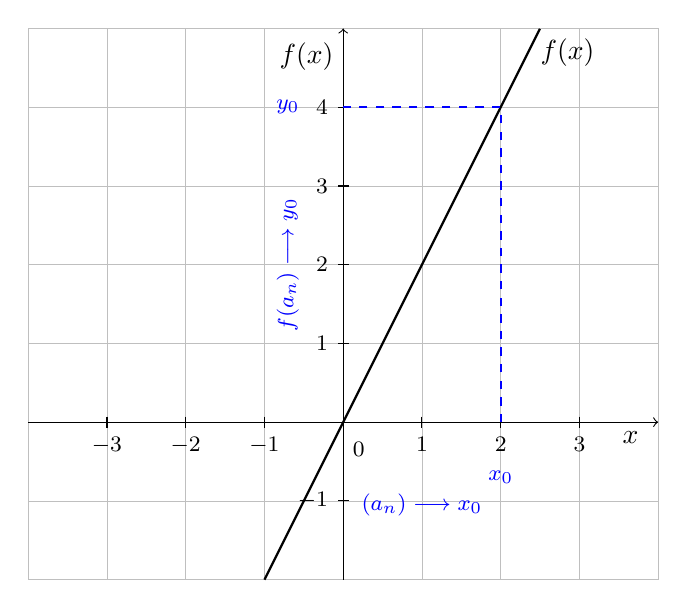
\begin{tikzpicture}
	
	% Gitternetzlinien
	\draw[xstep=1cm, ystep=1cm, very thin, color=lightgray] (-4,5) grid (4,-2);
	% x-Achse
	\draw[->] (-4,0) -- (4,0) node[below,xshift=-1em] {$x$}; 
	%Zahlen auf x-Achse
	\foreach \x in {-3,...,-1}
	\draw[shift={(\x,0)},color=black] (0pt,2pt) -- (0pt,-2pt) node[below] {\footnotesize $\x$};
	\foreach \x in {1,...,3}
	\draw[shift={(\x,0)},color=black] (0pt,2pt) -- (0pt,-2pt) node[below] {\footnotesize $\x$};
	% y-Achse 
	\draw[->] (0,-2) -- (0,5) node[left,yshift=-1em] {$f(x)$};%node[above left]
	%Zahlen auf y-Achse
	\foreach \y in {-1,...,-1}
	\draw[shift={(0,\y)},color=black] (2pt,0pt) -- (-2pt,0pt) node[left] {\footnotesize $\y$};
	\foreach \y in {1,...,4}
	\draw[shift={(0,\y)},color=black] (2pt,0pt) -- (-2pt,0pt) node[left] {\footnotesize $\y$};
	%Ursprung
	\draw[color=black] (0pt,-10pt) node[right] {\footnotesize $0$};
	
	
	
	\draw[thick,color=black] plot[samples=200, domain=-1:2.5] 
	(\x,{2*\x}) node[below, xshift=1em]{$f(x)$};
	
	\draw[color=blue] (2,0) node[yshift=-20] {\footnotesize $x_0$};
	\draw[color=blue] (1,0) node[yshift=-30] {\footnotesize $(a_n)\longrightarrow x_0$};
	\draw[color=blue] (0,4) node[xshift=-20] {\footnotesize $y_0$};
	\draw[color=blue] (0,2) node[xshift=-20,rotate=90] {\footnotesize $f(a_n)\longrightarrow y_0$};
	\draw[color=blue,dashed,thick] (2,0)--(2,4)--(0,4);
	\end{tikzpicture}\\
\end{center}
Linksseitiger Grenzwert:\\
\begin{align*}
\lim\limits_ {x\to\infty} f(x)=\lim\limits_ {\substack{x\to\infty\\x<x_0}}f(x)=y_0
\end{align*}
Rechtsseitiger Grenzwert:\\
\begin{align*}
\lim\limits_ {x\to\infty} f(x)=\lim\limits_ {\substack{x\to\infty\\x>x_0}}f(x)=y_0
\end{align*}
Beispiel:\\
\textbullet \;\; Linksseitiger Grenzwert von: $ \lim\limits_ {\substack{x\to\infty\\x<0}}\frac{2|x|}{x} $\\
\begin{align*}
\lim\limits_ {\substack{x\to\infty\\x<0}}\frac{2|x|}{x}=\lim\limits_ {x\to\infty}\frac{2(-x)}{x}=-2\\
\end{align*}
\textbullet \;\; Rechtsseitiger Grenzwert von: $ \lim\limits_ {\substack{x\to\infty\\x>0}}\frac{2|x|}{x} $\\
\begin{align*}
\lim\limits_ {\substack{x\to\infty\\x>0}}\frac{2|x|}{x}=\lim\limits_ {x\to\infty}\frac{2(x)}{x}=2\\
\end{align*}
%\subsection{Einseitige Grenzwerte-Teil II}
\href{https://youtu.be/KLn2p_dOASs}{Video 06}\\
\underline{Satz:}\\
\begin{center}

\fbox{\parbox  {128mm} {Existieren $ \lim\limits_ {\substack{x\to x_0\\x<x_0}}=a $ und $ \lim\limits_ {\substack{x\to x_0\\x>x_0}}=b $ und gilt $ a=b $, dann existiert auch:\\
		 \begin{center}
		 	 $ \lim\limits_ {x\to x_0}f(x)=a $
		 \end{center}}}
\end{center}
\vspace*{4mm}
\newpage
\noindent
Beispiel:\\
\textbullet \;\;$\lim\limits_ {x\to 0} \frac{2|x|}{x} $\\
$ \lim\limits_ {\substack{x\to 0\\x<0}}\frac{2(-x)}{x}=-2\neq 2=\lim\limits_ {\substack{x\to 0\\x>0}}\frac{2x}{x}\Rightarrow \lim\limits_ {x\to 0} \frac{2|x|}{x}$ existiert nicht \vspace*{2mm}\\
\textbullet \;\; $  \lim\limits_ {\substack{x\to 0\\x<0}}|x| $\\
\begin{quote}
	$  \lim\limits_ {\substack{x\to 0\\x<0}}|x|=\lim\limits_ {x\to 0}(-x) =0$\\
	$  \lim\limits_ {\substack{x\to 0\\x>0}}|x|=\lim\limits_ {x\ 0}  x=0$\\
	$\Rightarrow \lim\limits_ {x\to 0}|x|=0$\\
\end{quote}
\textbullet \;\; $ \lim\limits_ {x\to 0}\frac{1}{x} $\\
\begin{quote}
	$ \lim\limits_ {\substack{x\to 0\\x<0}}\frac{1}{x}=-\infty $ hat keinen Grenzwert, geht in das negative Unendliche.\\
	$ \lim\limits_ {\substack{x\to 0\\x>0}}\frac{1}{x}=\infty $ geht in das positive Unendliche\\
	$ \Rightarrow \lim\limits_ {x\to\ 0}\frac{1}{x}$ existiert nicht.
	\begin{center}
		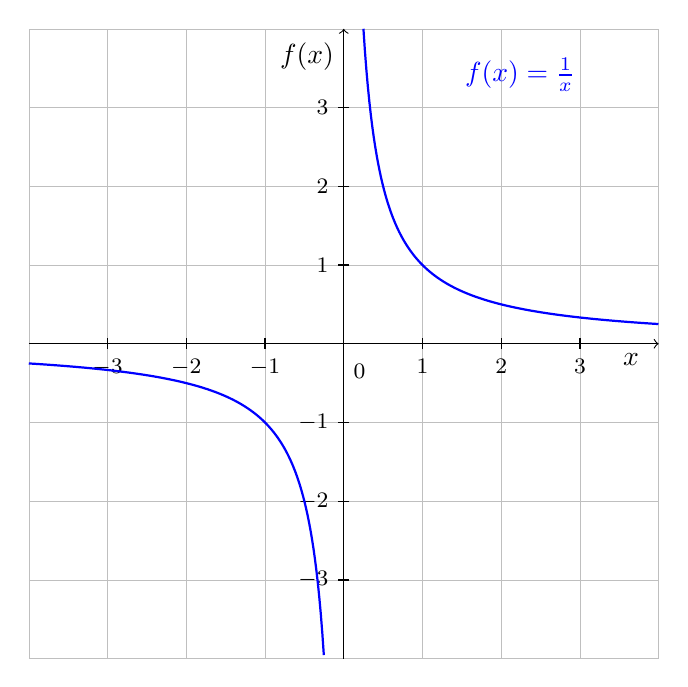
\begin{tikzpicture}
		
		% Gitternetzlinien
		\draw[xstep=1cm, ystep=1cm, very thin, color=lightgray] (-4,4) grid (4,-4);
		% x-Achse
		\draw[->] (-4,0) -- (4,0) node[below,xshift=-1em] {$x$}; 
		%Zahlen auf x-Achse
		\foreach \x in {-3,...,-1}
		\draw[shift={(\x,0)},color=black] (0pt,2pt) -- (0pt,-2pt) node[below] {\footnotesize $\x$};
		\foreach \x in {1,...,3}
		\draw[shift={(\x,0)},color=black] (0pt,2pt) -- (0pt,-2pt) node[below] {\footnotesize $\x$};
		% y-Achse 
		\draw[->] (0,-4) -- (0,4) node[left,yshift=-1em] {$f(x)$};%node[above left]
		%Zahlen auf y-Achse
		\foreach \y in {-3,...,-1}
		\draw[shift={(0,\y)},color=black] (2pt,0pt) -- (-2pt,0pt) node[left] {\footnotesize $\y$};
		\foreach \y in {1,...,3}
		\draw[shift={(0,\y)},color=black] (2pt,0pt) -- (-2pt,0pt) node[left] {\footnotesize $\y$};
		%Ursprung
		\draw[color=black] (0pt,-10pt) node[right] {\footnotesize $0$};
		
		\draw[thick,color=blue] plot[samples=200, domain=0.25:4] 
		(\x,{1/\x}) node[xshift=-5em,yshift=90] {$f(x)=\frac{1}{x}$};
		
		\draw[thick,color=blue] plot[samples=200, domain=-4:-0.25] 
		(\x,{1/\x}) ;
		
		
		
		\end{tikzpicture}\\
	\end{center}
\end{quote}
\subsubsection{Aufgabe zum Thema Einseitige Grenzwerte}
\href{https://youtu.be/3QFihiHQzq0}{Video 07}\\
Geben eine Funktion:  $f(x) =     \left\{ \begin{array}{lll}
	x^4-1&\mbox{für} & x>1\\
	x^2 &\mbox{für} & x\leq 1 \\
	
\end{array}\right.$\;\;\;\;$ x\in\mathbb{R} $\\
Überprüfe die Grenzwerte:\\
\begin{tabular}[t]{lll}% l=linksbündig r=rechtsbündig
	(i) & $ \lim\limits_ {x\to -1}f(x) $  \\
	(ii) & $ \lim\limits_ {x\to 1}f(x) $ \\	
\end{tabular} \vspace*{2mm}\\
(i) \;\;$\lim\limits_ {x\to -1}f(x)$\\
\begin{quote}
	\textbullet \;\; $ \lim\limits_ {\substack{x\to -1\\x<-1}}f(x) =\lim\limits_ {x\to -1}x^2=1$\\
	\textbullet \;\;$ \lim\limits_ {\substack{x\to -1\\x>-1}}f(x) =\lim\limits_ {x\to -1}x^2=1$\\
	Da beide einseitigen Grenzwerte exestieren und gleich sind, gilt hier $ \lim\limits_ {x\to -1}f(x)=1 $\\
\end{quote}
(ii) \;\;$\lim\limits_ {x\to 1}f(x)$\\
\begin{quote}
	\textbullet \;\; $ \lim\limits_ {\substack{x\to 1\\x<1}}f(x) =\lim\limits_ {x\to 1}x^2=1$\\
	\textbullet \;\; $ \lim\limits_ {\substack{x\to 1\\x>1}}f(x) =\lim\limits_ {x\to 1}x^4-1=0$\\
	Da beide einseitigen Grenzwerte verschieden sind existiert $ \lim\limits_ {x\to\ 1}f(x) $ nicht.\\
\end{quote}
\begin{center}
 $f(x) =     \left\{ \begin{array}{lll}
x^4-1&\mbox{für} & x>1\\
x^2 &\mbox{für} & x\leq 1 \\

\end{array}\right.$\\
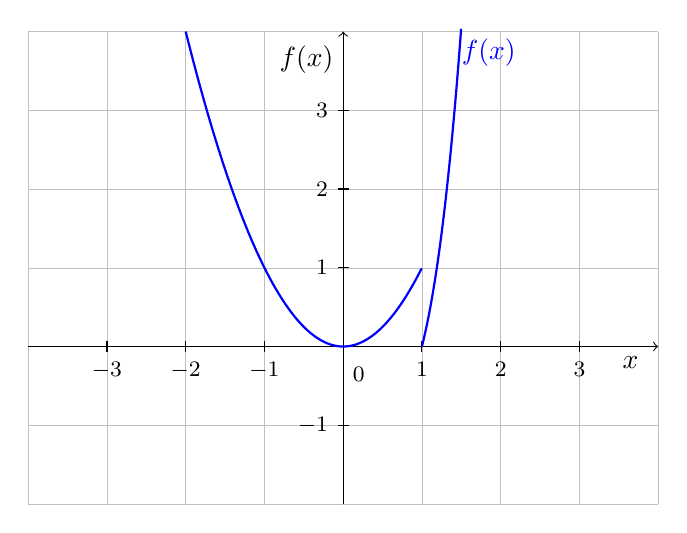
\begin{tikzpicture}

% Gitternetzlinien
\draw[xstep=1cm, ystep=1cm, very thin, color=lightgray] (-4,4) grid (4,-2);
% x-Achse
\draw[->] (-4,0) -- (4,0) node[below,xshift=-1em] {$x$}; 
%Zahlen auf x-Achse
\foreach \x in {-3,...,-1}
\draw[shift={(\x,0)},color=black] (0pt,2pt) -- (0pt,-2pt) node[below] {\footnotesize $\x$};
\foreach \x in {1,...,3}
\draw[shift={(\x,0)},color=black] (0pt,2pt) -- (0pt,-2pt) node[below] {\footnotesize $\x$};
% y-Achse 
\draw[->] (0,-2) -- (0,4) node[left,yshift=-1em] {$f(x)$};%node[above left]
%Zahlen auf y-Achse
\foreach \y in {-1,...,-1}
\draw[shift={(0,\y)},color=black] (2pt,0pt) -- (-2pt,0pt) node[left] {\footnotesize $\y$};
\foreach \y in {1,...,3}
\draw[shift={(0,\y)},color=black] (2pt,0pt) -- (-2pt,0pt) node[left] {\footnotesize $\y$};
%Ursprung
\draw[color=black] (0pt,-10pt) node[right] {\footnotesize $0$};

\draw[thick,color=blue] plot[samples=200, domain=-2:1] 
(\x,{\x*\x});

\draw[thick,color=blue] plot[samples=200, domain=1:1.5] 
(\x,{(\x*\x*\x*\x)-1}) node[below, xshift=1em]{$f(x)$};





\end{tikzpicture}\\
\end{center}
